\chapter{Implementation}

\label{chap:impl}

% -------------------------------------------------------------------------------------------------
%                                           General TODOs
% -------------------------------------------------------------------------------------------------


\todo{Add references to documentation at appropiate places}
\todo{ add disclaimer, that most of this information was derived from reading the source code and may in some places not be accurate because the code is pretty complex and
    i have only been at it for a few months}

% TODO viruteller address raum eines xv6 processes
% Qemu implementation TLB vs Echter TLB
% -------------------------------------------------------------------------------------------------
%                                    Chapter structure overview
% -------------------------------------------------------------------------------------------------

%   Source overview
%     QEMU
%     xv6
%   Stage1 - Single Fixed address
%     Qemu - exception
%     xv6 - tlb triggerer
%   Stage2 - VM PTW with TLB miss handler
%     Qemu -> Extension to all addresses, csr
%     xv6 -> tlb miss handler
%       Exception vector entry -> state save, kernel stack
%   Stage3 - Dynamic Segmentation allocation scheme (btw -> link to MIPS?)
%     Qemu -> No more changes needed
%     xv6 -> A lot of changes here
%   Debugging
%   Discussion on implementation
%       Concurrency
%       VM Features
% -------------------------------------------------------------------------------------------------

% High level description of the development steps and their reasoning

% -------------------------------------------------------------------------------------------------
% Section on the rationale for choosing this platform -> or just say that this was chosen and dont rationalize it

\section{Programming Platform}
\subsection{QEMU}
The \texttt{softtlb} design approach requires the CPU to throw an exception when the TLB misses. There is
currently neither a RISC-V platform that supports nor a extension to the RISC-V that specifies that behavior.\\
The logical consequence is to use an emulator and implement the required functionality.\\
This paper uses the QEMU emulator as a foundation for the implementation. QEMU supports a big range of
different platforms and is thus not the simplest source to modify. Additionally, detailed documentation
on internal structures is sparse.\\
However, QEMU does support a lot of features and extensions of the RISC-V target and is quite performant
\cite{bellard2005QEMU}.

% -------------------------------------------------------------------------------------------------

%This section is important for the rationale on choosing a format of the CSRs
%Vielleicht sollte dieser Teil einfach erst im hinblick auf replacement policies Dikutiert werden
% In meinem Programmiermodell ist ja der TLB nichts weiter als ein Indiziertes array von daten, 
% Weitere Aspekte sind ja hier erst mal out of scope
\subsubsection{TLB}
% What type of cache modeled? - direct mapped, associative?

\todo{description of QEMU TLB structure in fundamentals, theory or implementation?}
% Does the QEMU tlb implementation impact the theory? -> It should not
%   It only has impact once we have to decide on a specific format for the tlbh and tlbl csrs
%   But I can put all the theoretical parts into theory, so ASID etc
%   and the modification of the theory based on concrete hardware can come into the impl chapter
%       -> mmuidx and stuff


% -------------------------------------------------------------------------------------------------


\subsection{xv6-riscv}
xv6 is a simple teaching operating system loosely following the design of Unix Version 6 \cite{cox2011xv6}.
It is used to teach an operating systems course and does not contain the complexities of real-life
operating systems.

% -------------------------------------------------------------------------------------------------
%                                    SECTION Source Description
% -------------------------------------------------------------------------------------------------
\section{Source Overview}
The implementation consists of two fundamental parts:
The extension of RISC-V ISA emulated by QEMU and the implementation of a
TLB Miss Handler.

% -------------------------------------------------------------------------------------------------

\subsection{QEMU}
\texttt{cputlb.c} found in \texttt{accel/tcg} contains the TLB-handling logic for all
emulation targets; from there, target-specific functions for TLB management are called.
The target-specific functions are implemented in \texttt{target/riscv}.\\
Every target needs to implement the functions in the \texttt{TCGCPUOps} struct in
\texttt{include/hw/core/tcg-cpu-ops.h}. This struct is part of the glue that connects the target-independent
Tiny Code Generator (TCG) backend with the target-specific functions and structures.

% -------------------------------------------------------------------------------------------------

\todo{sequence diagram for function calls accross the QEMU repository}

% -------------------------------------------------------------------------------------------------

% TCGCPUOps struct
% TODO Ausgangspunkt sollte die mmu_lookup1 funktion sein!
The \texttt{TCGCPUOps} struct includes a function pointer named \texttt{tlb\_fill}. The function is called
when MMU lookups to the TLB and QEMU's victim TLB fail.
For the riscv target, the function \texttt{riscv\_cpu\_tlb\_fill} is assigned to the \texttt{tlb\_fill}
function pointer in \texttt{target/riscv/tcg/tcg-cpu.c}.\\
The implementation for \texttt{riscv\_cpu\_tlb\_fill} is in \texttt{target/riscv/cpu\_helper.c}. This is a common
file to be found in a target-specifc directory and contains general functionality to implement the \texttt{TCGCPUOps} struct.\\


\todo{explain PTE}

% -------------------------------------------------------------------------------------------------

\subsection{xv6}



% -------------------------------------------------------------------------------------------------
%                                END OF SECTION - Source Description
% -------------------------------------------------------------------------------------------------




% First step in the development process
% -------------------------------------------------------------------------------------------------
%                                          SECTION STEP 1
% -------------------------------------------------------------------------------------------------
\section{TLB miss handling for a single fixed address}

% Why only start with one fixed address?
Changing the whole system to start throwing a TLB\_MISS Exception on every virtual address would
make it very hard to debug both first tries at implementing a handler for the exception and the
exception throwing code in QEMU itself.
And not only would the exception be thrown as soon as virtual memory is activated in
\texttt{xv6-riscv:kernel/main.c}, the exception would be thrown
as soon as exceptions are activated and a memory access happens, because QEMU also uses the
\texttt{fill\_tlb} routine to fill the TLB with direct
virtual-to-physical mappings when no virtual memory is used. This speeds up the execution of
the dynamically-translated code, as it can directly
lookup addresses in the TLB using a fast path.\\ \todo{add: dynamically-generated tcg code can
    directly use the TLB structures}
To properly test the implementation, the \texttt{tlb\_fill} function was replaced to throw the
TLB\_MISS exception for
one specified, page-aligned address and to continue on normally for every other address.
The implementation is outlined
in Listing \ref{lst:specialCaseTLBfill}.

% -------------------------------------------------------------------------------------------------

\subsection{QEMU}
%TODO Explain what the riscv_cpu_tlb_fill function does originally - in detail
% TODO discussion and reference to READER/SPECIFICATION on what exception numbers and other constants can be used and are free

% Qemu RISCV  exception adding "tutorial"
%TODO Description of the TLB Exception implementation and how to generally add exceptions to the QEMU plattform
% TODO List of code locations where changes need to be added -> should be usable as back reference for implementing more exceptions

% -------------------------------------------------------------------------------------------------

% This section describes the necesarry steps for adding the tlb miss exception to the qemu source
%in comparison with Page fault exceptions
\subsection{Adding the TLB MISS exception}
The required behavior for the TLB Miss exception is similar to the behavior of a page fault exception.
The RISC-V Instruction Set Manual: Volume II \cite{RISCVInstructionSet} describes when page faults
are triggered in the virtual address translation process. Page faults are thrown when:
\begin{itemize}
    \item the valid bit of a PTE is 0; the read bit is 0 and the write bit is 1; any of the reserved
          bits is set
    \item the PTE at the last level of the page table tree does not the read or execute bits set.
    \item the requested memory access type is not allowed by the read, write, execute and user bits.
    \item the PTE describes a missaligned superpage.
\end{itemize}
Depending on active extensions, there are possibly more scenarios where page faults are triggered.\\
The page fault will then make the operating system jump to a specific location in the kernel code
specified by the (physical) address found in the \texttt{mtvec} register.\\
The TLB Miss exception does not have to trigger in the same situations as the page fault exception,
but rather before the page table is traversed by the emulated hardware pagetable-walker.
However, the code for the page fault exceptions gives hints for where changes need to be made in the QEMU
source to add a custom exception.\\ % Now: Which places need to be changed?

% -------------------------------------------------------------------------------------------------

% -------------------------------------------------------------------------------------------------

% Adding new Exception to Qemu RV target
\paragraph{Adding a new exception}to the QEMU emulator requires changes at a number of places. In the following,
the relevant code locations in the QEMU source are shown.\\
This may be completely different for other targets, as the exception code is mostly target specific and
this implementation only looked at the RISC-V target.
\begin{itemize}
    \item \texttt{target/riscv/cpu\_bits.h} contains all CPU-definitions specific to the RISC-V target.
          There is also a enum called \texttt{RISCVException} which contains the number-codes for all RISC-V exceptions.
          In choosing a appropiate number for a new exception, one should consult the Privileged Architecture Specification \cite{RISCVInstructionSet}.
          There are specific exception code ranges that are designated for custom use. E.g. the codes 24--32 and 48--63.
    \item \texttt{target/riscv/cpu\_helper.c\:riscv\_cpu\_do\_interrupt\(\)} is the target-specific function
          for triggering interrupts. Here it suffices to add the new exception enum item to the switch case, when
          the new exception is similar in behavior to exising exceptions.\\
          Here the new exception is simply supposed to jump into an exception handler in the kernel. A lot of exceptions
          like page faults share that behavior.
    \item Finally, if the exception should be delegatable to supervisor mode or user mode, the n-th bit,
          with n being the exception code, needs to be set in the \texttt{DELEGABLE\_EXCPS} definition in \texttt{target/riscv/csr.c}.
          This enables the kernel to delegate the exception to another priviledge level by setting the appropiate
          bit in the \texttt{medeleg} and \texttt{sedeleg} CSRs.
\end{itemize}

% -------------------------------------------------------------------------------------------------


% \subsection{CSR Modifications}
% \subsubsection{TLB Modification via CSR}
% \subsubsection{Switching between HW and SW TLB miss handling}

\subsection{xv6}
% TODO TLB exception trigger


% -------------------------------------------------------------------------------------------------
%                                       END OF SECTION - STEP 1
% -------------------------------------------------------------------------------------------------



% Second step: Extending the tlb miss handling to be used for all addresses -> implementing a softvm ptw
% -------------------------------------------------------------------------------------------------
%                                         SECTION - STEP 2
% -------------------------------------------------------------------------------------------------
\section{Software page table walk and TLB filling}


\subsection{QEMU}

% -------------------------------------------------------------------------------------------------


%Implementation of CSRs

%   Choosing a CSR number -> back reference to theory section on CSRs

\subsection{Adding new CSRs for writing TLB entries}

% More controll with further CSRs -> MIPS comparison
%\section{Further possible extensions to the TLB CSRs}
\todo{typical tlb replacement strategies}
\todo{How does QEMU replace TLB entries -> index?} % Direct mapped
With the new CSRs presented above, it is possible to write TLB entries.
The placement of the entry and thus the entry to be replaced can not be selected.
The replacement policy would be completely up to the hardware implementation.
It would also be possible to further extend the ISA with additional CSRs to
support specific selection of entries to be replaced, or to select between
a number of replacement strategies.
However, the efficiency of more complex strategies need to be weighed carefully
against their benefits, since the TLB filling is on the critical path of all
memory accesses.


\todo{discussion of implementation at the end of this chapter: shortcommings, comparison QEMU - MIPS, comparison xv6 new vm - other vm -> eval??}

% -------------------------------------------------------------------------------------------------


\subsection{xv6}
% TODO TLB fill manager

% Previous state of xv6 machine mode trap handler
%   -> Only for Timer Interrupt
%   -> Small amount of saved registers

% Changes -> Vectored mode to keep timer interrupt as is, just need to move it

% -------------------------------------------------------------------------------------------------
%                                       END OF SECTION - STEP 2
% -------------------------------------------------------------------------------------------------


% Third step: Dynamic Segmented memory with a simple function and no page table
% -------------------------------------------------------------------------------------------------
%                                       STEP 3 - New VM
% -------------------------------------------------------------------------------------------------
\section{Software-controlled virtual memory without a page table}
\subsection{QEMU}

% -------------------------------------------------------------------------------------------------


\subsection{xv6}
% MODULEs and Systemcalls of xv6 to be discussed
% \section{Relevant Modules in the xv6 Source}
% \paragraph*{kalloc - physical memory allocator}
% \paragraph*{proc}
% \paragraph*{vm.c}
% \subsection*{Syscalls to change}
% System call interface should stay the same so that existing processes can continue
% as usual -> new virtual memory scheme should be completely transparent%
%\paragraph*{fork}
% creating a new addresse space -> fixed number of processes ? ?
%\paragraph*{exit}
% freeing memory?
%\paragraph*{exec}
% same as fork?
%\paragraph*{sbrk}
% allocating new memory
Sbrk is the system call with which a program can change its program break. The program break
is the end of the programs data segment. This system call is typically used to either
increase or decrease a programs memory.
Sbrk would typically be called by the memory manager of the user program. Calls
to malloc would for example call sbrk when there is not enough memory available to
satisfy the call to malloc.
Internally, sbrk calls a function called growproc(n) which grows or shrinks to calling
processes memory by n bytes.
growproc will then call either uvmalloc() or uvmdealloc(). These functions need to be
changed to use the new allocation scheme.

% -------------------------------------------------------------------------------------------------
% -------------------------------------------------------------------------------------------------

\section{Simplest Case: Fixed memory area for each process}
\subsection{Address Spaces}
The available physical memory is split into evenly sized portions, from now called address space.
When a new process is started it tries to acquire an address space by checking whether
there is a free one and then claiming that free address space.
The number of address spaces will thus limit the number of concurrently running programs.
Why not just use the Pids and reuse them? The order of termination is not clear, bookkeeping
may be expensive. PID range is typically a lot bigger -> But this can be limited.
\subsection{Discussion: Limitations}
This is not really virtual memory and works only, because xv6 just added more memory at the low
end of the address space. No mappings are made in between or at high addresses.
This is where a hash function could come in handy. However collisions and access rights and
collision detection \ldots
Verification via % \texttt{\verbatim{readelf -l user/\_*}}
shows that all vaddr are in the low addresses.



% -------------------------------------------------------------------------------------------------




% Final allocation scheme
% TODO this might actually describe an intermediate allocation scheme
\paragraph*{Experimental Allocation Scheme}
xv6 keeps all of its unused physical memory in a linked list. The linked list itself is stored
in the free blocks, as they are not used for anything else. When a process asks for more memory
the kalloc() function retrieves the first element from the linked list, updates the head
of the list to point to the next element and returns the pointer to the first element,
which is the same as the physical address for the page managed by that first list item.
kalloc() is called by the uvmalloc() function, and since we want to change the way
the virtual memory management works, it would make sense to directly change the uvmalloc() function.
However, in order to properly test the physical memory allocation first, we will change
the allocation scheme first and then the mapping, as the trampoline page would not work anymore.

The new allocation scheme statically assigns a fixed portion of the available physical memory
to each process. The size is determined by the size of physical memory and the maximum number
of processes.
kalloc() will then use the process id, the current size of the process and the requested
increase in size to determine the next page for the process.
\todo{assumptions on the process model -> allocation works only for processes that grow linearily and do not use pages in between or at the top}

% discussion on the new allocation scheme -> 
\subsection*{Why does this not work for anything else but the sbrk syscall}
- kalloc with sbrk uses the current process size to determine the next free space in
the address space of the process
- The processes size only keeps track of the text data and so on segments. So only stuff
the program is aware of. Page table pages need to be allocated per process as well but
do not contribute to the overall size of the process so they can not be put into the
processes memory space. This has the direct advantage that users can not access their page tables
but this was never the problem because pages containing page tables could simply be marked
as not user accessible. And of course this brings some disadvantages: Kernel size becomes
a scarce resource and user address spaces are not self contained anymore, page tables now reside
somewhere else entirely.
But since it is the goal to get rid of page tables anyways, its not too big of a problem.
When we get rid of the page tables, we get rid of a huge part of the tables that can not
be directly allocated using the respective process size.
What are the other pages and allocations that can not rely on the processes size?

One further problem is that deallocation is not working. But in principle, all pages belonging
strictly to one process can be allocated on this sort of stack. The size counter
needs to be adapted to not only account for the processes own memory, but also
for all the memory that is allocated for the process.

% -------------------------------------------------------------------------------------------------

% \section{Changing physical memory allocation}
% \subsection{Special cases}
% \paragraph*{Kernel direct mapping}
% \paragraph*{MMIO}
% \paragraph*{Trampoline}


% -------------------------------------------------------------------------------------------------
%                                    END OF SECTION - Step 3
% -------------------------------------------------------------------------------------------------



% TODO Should this be an appendix?
% -------------------------------------------------------------------------------------------------
%                                         SECTION - Debugging
% -------------------------------------------------------------------------------------------------

\section{Debugging}
Wenn man gleichzeitig Änderung am Qemu Emulator und an xv6 durchführt, kann es schwierig sein
herauszufinden wo der Fehler liegt. Hier wird zunächst einmal beschrieben wie man Qemu und
xv6 einzeln debuggen kann und darauf wird ein gemeinsamer Debugging Prozess aufgezeigt.
Das kann zum Beispiel nützlich sein wenn man versucht den Code Pfad zwischen Software und
Emulierter Hardware nachzuverfolgen.\\
Hier wird keine Anleitung zum benutzen von GDB geliefert, sondern nur ein paar eigenheiten
und tricks die beim debuggen des Codes für diese Arbeit nützlich waren. Vielleicht sind
diese ja auch in anderen Szenarios nützlich.
\subsection{xv6}
Das Makefile im xv6-riscv source repository verfügt über die Regel qemu-gdb um xv6 in qemu
mit einem GDB server zu starten. In einem anderen Terminal kann man dann gdb mit der binary
die man debuggen möchte starten und dann mit \texttt{target remote:<port>} eine verbindung
zum gdbstub herstellen.\\
Ein Kommentar im makefile legt zwar nahe, dass die Makefile rule zum Debuggen vom user mode
gedacht ist, aber tatsächlich hält einen nichts auf auch den kernel zu debuggen. Das ist
für Änderungen am Memory system auch sehr nützlich.\\
\textbf{Debugging user mode} Für das debuggen eines user mode programms will man oft bei
der main Funktion anfangen. Breakt man auf die Funktion wird ein Breakpoint auf eine eine recht
niedrige virtuelle Addresse gesetzt. Hat man den Breakpoint schon gesetzt bevor man überhaupt
den Kernel gestartet hat kann es dann beim start sein, dass man direkt wieder stoppt.
Das liegt dann daran, dass man sich gerade im Qemu boot ROM befindet, der von Qemu in
das emulierte Memory Layout in den Bereich von \texttt{0x0 - 0x1000} gemappt wurde.
Der debugger unterscheidet hier nicht zwischen virtuellen und physischen Addressen und
schaut lediglich was im PC steht.
\todo{das satp PPN field könnte noch für weitere infos benutzt werden (Konfiguration der vm für den process)}

\textbf{Debugging the kernel} Nach dem ersetzen des virtuellen Memorysystems hat sich beim
debuggen des Kernels ein interessanter effekt bemerktbar gemacht: Sobald in der
\texttt{kvminithart()} funktion das \texttt{satp} register gesetzt wird kann GDB den code zu der
aktuellen addresse (und allen folgenden) anzeigen.\\
Das ist dem Wert des \texttt{satp} registers geschuldet. Nach dem Umbau des VM systems enthält
dieses nicht mehr die \texttt{PPN}. Nur noch das \texttt{MODE} und \texttt{ASID} Feld sind
für das neue system von bedeutung. Es gibt auch gar keine Page table mehr auf die die PPN zeigen
könnte.\\
Dieses Verhalten lässte vermuten, dass der von qemu implementierte GDBstub den hardware-emulierten
page walk macht um an die physischen addressen und damit an den Code zu kommen. Das funktioniert
natürlich nicht ohne page table.\\
Eine Möglichkeit den kernel wieder ordentlich in gdb debuggen zu können, wäre es die kernel
page table wieder so wie zuvor aufzubauen. Da aber die mappings im Kernel alle direkte mappings
sind, reicht es auch einen PTE für die addresse \texttt{0x80000000} bei der der kernel code
anfängt, hinter der PPN in \texttt{satp} abzulegen.\\
% wie muss der PTE aussehen?
Im Code wurde dafür eine ganze Page wie folgt allokiert:
\begin{lstlisting}[language=c,float=h!,
    label={lst:fake_pt}]
    uint64 *pt = (uint64*)kalloc();
    for(uint64 i = 0 ; i < 512; i++) {
      pt[i] = 0xffffffffffffffff;
    }
    pt[2] = ((0x80000000 >> 2)| PTE_V | PTE_X | PTE_W | PTE_R);
\end{lstlisting}
Es würde allerdings auch reichen nur den Platz für einen einzelnen PTE
zu allokieren. Die PPN muss allerdings dann so gesetzt werden,
dass mindestens der Eintrag bei Index 2 vorhanden ist. Interpretiert man
die Adresse \texttt{0x80000000} als virtuelle Addresse, so ergibt sich
nämlich für das \texttt{VPN[2]} Feld der Wert 2.\\
Setzt man diesen Top-level page table entry als valide, so wird der Speicher
an dieser Stelle 1 GB Superpage behandelt. Das reicht aus um den Kernelcode
abzudecken und der Code kann beim Debuggen wieder wie gehabt gesehen werden.

\subsection{QEMU Monitor}
Mit dem Qemu monitor lassen sich allerlei informationen über die laufende
emulation anzeigen lassen. Besonders interessant für diese Arbeit wäre der
monitor für die aktuell im emulierten TLB enthaltene Mappings. Gerade für
RISC-V war dieser allerdings nicht verfügbar.
\todo{Beschreibung der TLB strukturen früher im kapitel}



% -------------------------------------------------------------------------------------------------
%                                    END OF SECTION - Debugging
% -------------------------------------------------------------------------------------------------


% -------------------------------------------------------------------------------------------------
% -------------------------------------------------------------------------------------------------
%                                           END OF CHAPTER
% -------------------------------------------------------------------------------------------------
% -------------------------------------------------------------------------------------------------



% -------------------------------------------------------------------------------------------------
%                                   STUFF THAT NEEDS TO BE SORTED IN
% -------------------------------------------------------------------------------------------------




% riscv_cpu_tlb_switch function 
%TODO is this listing really interesting?
\begin{lstlisting}[language=c,float=h!,
    caption={Alternative Implementation for the RISC-V tlb\_fill function with a special case to start testing TLB Miss Handler implementations},
    label={lst:specialCaseTLBfill}]
bool my_riscv_cpu_tlb_fill(CPUState *cs, vaddr address, int size,
    MMUAccessType access_type, int mmu_idx,
    bool probe, uintptr_t retaddr)
{
    RISCVCPU *cpu = RISCV_CPU(cs);
    CPURISCVState *env = &cpu->env;
    int mode = mmuidx_priv(mmu_idx);
    int vm = get_field(env->satp, SATP64_MODE);
    bool ret = false;

    if(!(vm == VM_1_10_MBARE || mode == PRV_M) &&
            address == (uint64_t)0x84fff000) {
        ret = riscv_cpu_tlb_miss_exception(cs,address,size,access_type, mmu_idx, probe, retaddr);
    } else {
        ret =  riscv_cpu_tlb_fill(cs,address,size,access_type, mmu_idx, probe, retaddr);
    }
    return ret;
}
\end{lstlisting}

.
% -------------------------------------------------------------------------------------------------


\begin{figure*}[ht!]
    \centering
    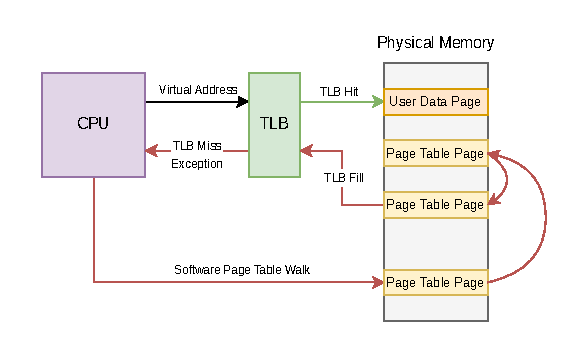
\includegraphics[scale=1.5]{figures/theory_sw_ptw.pdf}
    \caption[Software Page Table Walker]{Instead of transfering control over to the MMU to fill in the missing mapping,
        the TLB Miss exception invokes a software page table walker}
    \label{fig:theory:sw_ptw}
\end{figure*}





\begin{figure*}[t]
    \centering
    \begin{bytefield}[bitwidth=\widefigurewidth/56,bitheight=\widthof{~PBMT~}, bitformatting={\tiny\bfseries}, boxformatting={\centering}]{56}
        \bitheader[endianness=big]{55,30,29,21,20,12,11,0} \\
        \bitbox{26}{PPN[2]} &
        \bitbox{9}{PPN[1]} &
        \bitbox{9}{PPN[0]} &
        \bitbox{12}{Page Offset}\\
    \end{bytefield}
    \caption[RISC-V Sv39 Physical Address]{RISC-V Sv39 Physical Address}
    \label{fig:theory:sv39pa}
\end{figure*}

\begin{figure*}[t]
    \centering
    \begin{bytefield}[bitwidth=\widefigurewidth/64,bitheight=\widthof{~PBMT~}, bitformatting={\tiny\bfseries}, boxformatting={\centering}]{64}
        \bitheader[endianness=big]{63,62,61,60,54,53,28,27,19,18,10,9,8,7,6,5,4,3,2,1,0} \\
        \bitbox{1}{N} &
        \bitbox{2}{\rotatebox{90}{PBMT}} &
        \bitbox{7}{Reserved} &
        \bitbox{26}{PPN[2]} &
        \bitbox{9}{PPN[1]} &
        \bitbox{9}{PPN[0]} &
        \bitbox{2}{\rotatebox{90}{RSW}} &
        \bitbox{1}{D} &
        \bitbox{1}{A} &
        \bitbox{1}{G} &
        \bitbox{1}{U} &
        \bitbox{1}{X} &
        \bitbox{1}{W} &
        \bitbox{1}{R} &
        \bitbox{1}{V}
    \end{bytefield}
    \caption[RISC-V Sv39 Page Table Entry]{RISC-V Sv39 Page Table Entry}
    \label{fig:theory:sv39pte}
\end{figure*}


\begin{figure*}[t]
    \centering
    \begin{bytefield}[bitwidth=\widefigurewidth/64,bitheight=\widthof{~PBMT~}, bitformatting={\tiny\bfseries}, boxformatting={\centering}]{64}
        \bitheader[endianness=big]{63,60,59,44,43,0} \\
        \bitbox{4}{Mode} &
        \bitbox{16}{ASID} &
        \bitbox{44}{PPN} \\
    \end{bytefield}
    \caption[RISC-V Sv39 \texttt{satp} CSR]{RISC-V Sv39 \texttt{satp} CSR}
    \label{fig:theory:sv39satp}
\end{figure*}



